\section{Correlation from Experiment Two}\label{app:cor_exp_two}

This section illustrated the correlation heatmap from \cref{subsec:exp_two}.

\begin{figure}[H]
    \centering
    \begin{subfigure}[b]{0.49\textwidth}
        \centering
        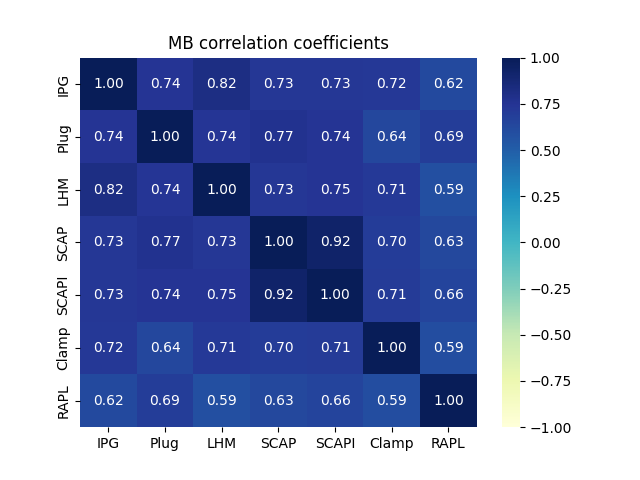
\includegraphics[width=\textwidth]{figures/MandelbrotDut1.png}
        \caption{DUT 1}
        % \label{fig:subfig1}
    \end{subfigure}
    \hfill
    \begin{subfigure}[b]{0.49\textwidth}
        \centering
        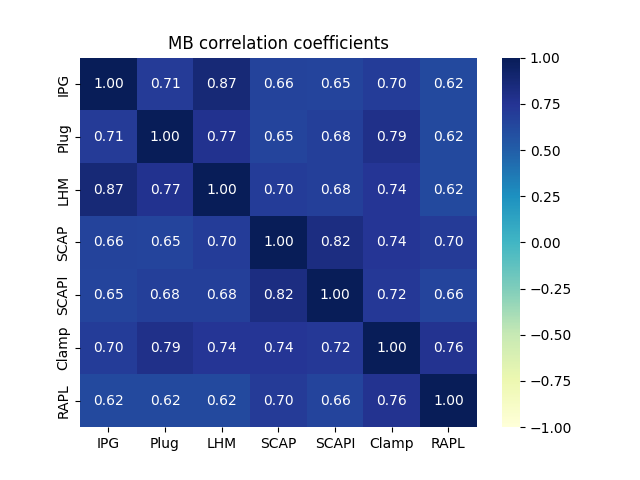
\includegraphics[width=\textwidth]{figures/MandelbrotDut2.png}
        \caption{DUT 2}
        % \label{fig:subfig2}
    \end{subfigure}
    \caption{Heatmap showing the correlation coefficient between all of the measurement instruments on Windows for the MB benchmark}
    % \label{fig:sidebyside}
\end{figure}

\begin{figure}[H]
    \centering
    \begin{subfigure}[b]{0.49\textwidth}
        \centering
        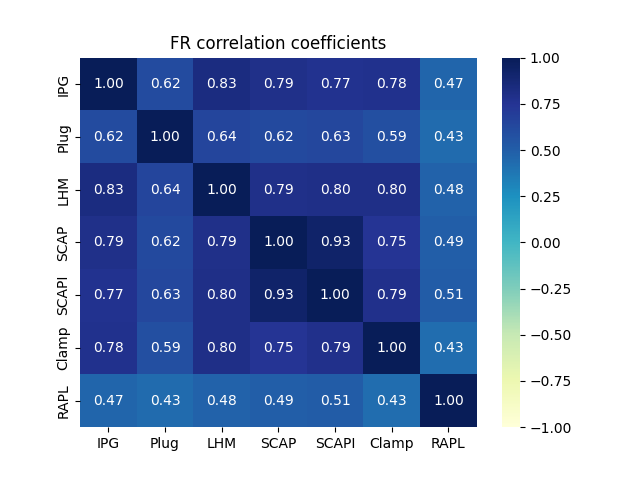
\includegraphics[width=\textwidth]{figures/Fannkuch-reduxDut1.png}
        \caption{DUT 1}
        % \label{fig:subfig1}
    \end{subfigure}
    \hfill
    \begin{subfigure}[b]{0.49\textwidth}
        \centering
        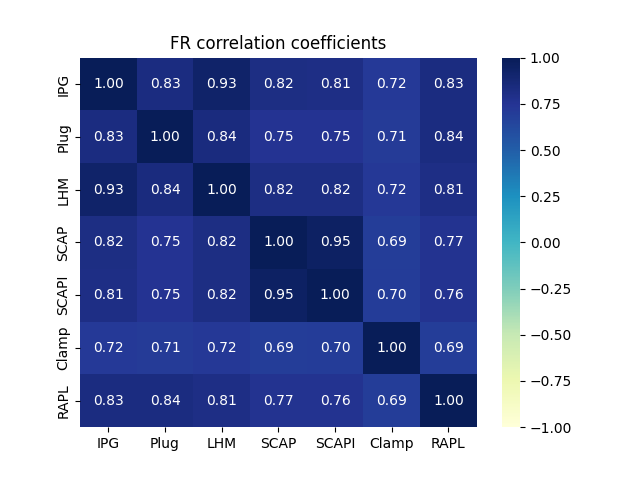
\includegraphics[width=\textwidth]{figures/Fannkuch-reduxDut2.png}
        \caption{DUT 2}
        % \label{fig:subfig2}
    \end{subfigure}
    \caption{Heatmap showing the correlation coefficient between all of the measurement instruments on Windows for the FR benchmark}
    % \label{fig:sidebyside}
\end{figure}

% \begin{figure}[H]
%     \centering
%     \hspace*{-1cm} % move the figure 1cm to the left
%     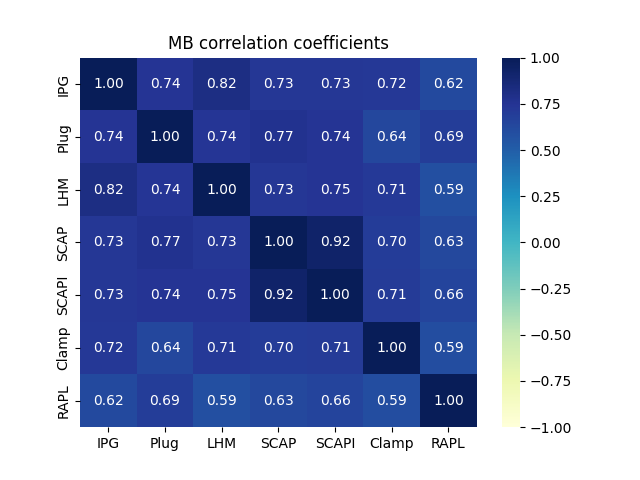
\includegraphics[width=0.6\textwidth]{figures/MandelbrotDut1.png}
%     \caption{Heatmap showing the correlation coefficient between all of the measurement instruments on windows for the MB benchmark for dut 1.}
%     \label{fig:mandelbrotCorrDut1}
% \end{figure}
% \begin{figure}[H]
%     \centering
%     \hspace*{-1cm} % move the figure 1cm to the left
%     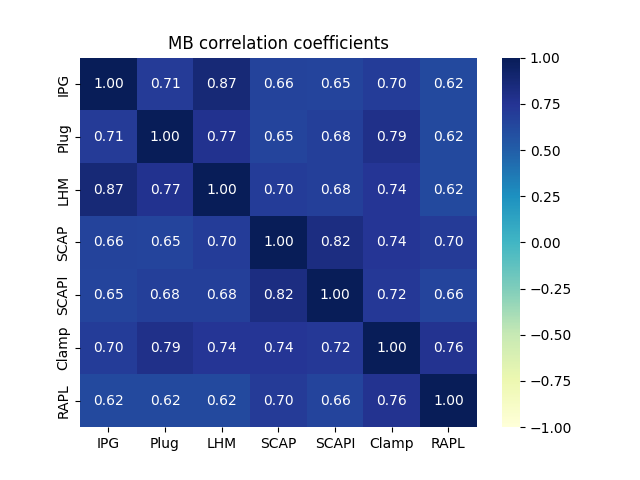
\includegraphics[width=0.6\textwidth]{figures/MandelbrotDut2.png}
%     \caption{Heatmap showing the correlation coefficient between all of the measurement instruments on windows for the MB benchmark for dut 2.}
%     \label{fig:mandelbrotCorrDut2}
% \end{figure}

% \begin{figure}[H]
%     \centering
%     \hspace*{-1cm} % move the figure 1cm to the left
%     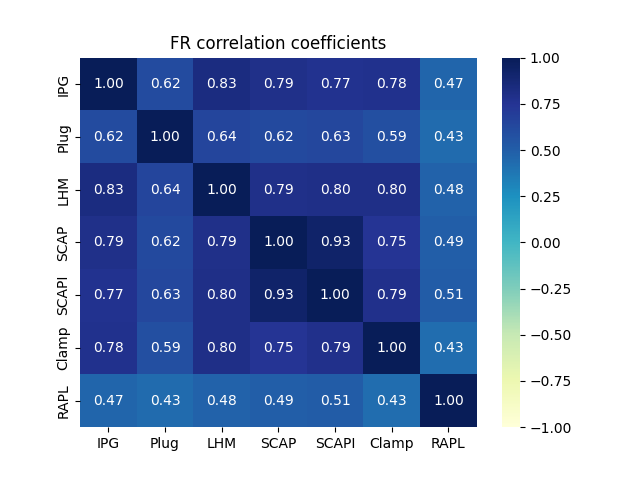
\includegraphics[width=0.6\textwidth]{figures/Fannkuch-reduxDut1.png}
%     \caption{Heatmap showing the correlation coefficient between all of the measurement instruments on windows for the FR benchmark for dut 1.}
%     \label{fig:FRCorrDut1}
% \end{figure}

% \begin{figure}[H]
%     \centering
%     \hspace*{-1cm} % move the figure 1cm to the left
%     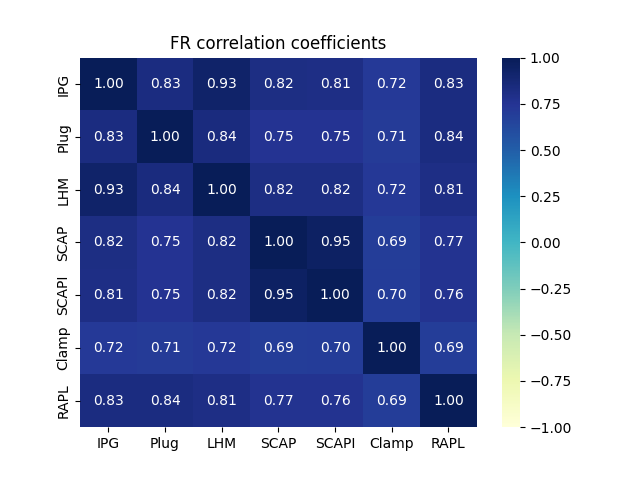
\includegraphics[width=0.6\textwidth]{figures/Fannkuch-reduxDut2.png}
%     \caption{Heatmap showing the correlation coefficient between all of the measurement instruments on windows for the FR benchmark for dut 2.}
%     \label{fig:FRCorrDut2}
% \end{figure}